\documentclass[oneside,openany]{amsdtx}
\usepackage[margin=.75in]{geometry}
\usepackage{graphicx,float,amsmath,amssymb,url,multicol,booktabs,bm,array,enumitem}
\usepackage[dvipsnames]{xcolor}
\usepackage[allcolors=black]{hyperref}
\usepackage[T1]{fontenc}
\usepackage[utf8]{inputenc}
\usepackage[english]{babel}
\usepackage{lmodern}
\usepackage{siunitx}
\usepackage{listingsutf8}
\definecolor{b}{HTML}{3C78D8}\definecolor{B}{HTML}{08357E}\definecolor{g}{HTML}{38761D}
\definecolor{r}{HTML}{7A0101}\definecolor{phenolic}{HTML}{A65A2E}\definecolor{aluminium}{HTML}{A8B0B8}
\newcolumntype{L}[1]{>{\raggedright\arraybackslash}p{#1}}
\protected\def\code#1{\texttt{\detokenize{#1}}}
\sisetup{locale=US,per-mode=symbol,range-phrase=--,range-units=single}
\setcounter{secnumdepth}{3}\setcounter{tocdepth}{2}
\title{~\\[-2em]\sc Preparation of Thermochemical Simulation v0\\
for the New Phenolic Liner}
\author{\sc MIT Rocket Team --- M. Nichitiu --- Solid Propulsion Simulations}
\date{\sc September 20, 2026}

\begin{document}
\selectlanguage{english}
\maketitle
\begin{multicols}{2}
{\color{white}.}~~~~~~~~~~~~~~~~~
\includegraphics[scale=0.1]{logos/rtlogo.pdf}\\[1em]
~\vspace{3.3em}~\\[-4.6em]{\color{white}.}~~~~~
\includegraphics[scale=0.2]{logos/ansys.png}
\end{multicols}
~\\[-1em]
\tableofcontents
\vfill
\begin{center}\begin{minipage}{0.96\textwidth}\small
\textbf{Purpose of this document.} This report records the reproducible
preparation of the first model version for the new motor. It strictly separates
the requested geometry from assumptions inherited from the earlier simulations.
The native Windows model, mesh, restart chain, and MAPDL preflight are ready,
but no transient calculation has been started. The primary goal is to compute,
without ambiguous terminology, removed phenolic thickness, remaining thickness,
pyrolysis-gas mass, and consumed-carbon mass at every time.
\end{minipage}\end{center}
\vfill

\section{Definition of the new motor}
\subsection{Imposed dimensions}
The brief supplied for this study contains three diameters:
\(D_{\mathrm{Al,out}}=\SI{6.000}{in}\),
\(D_{\mathrm{Al,in}}=D_{\mathrm{ph,out}}=\SI{5.625}{in}\), and
\(D_{\mathrm{ph,in}}=\SI{5.250}{in}\). Unlike the first two historical
simulations, these dimensions are correctly treated as \emph{diameters} and
divided by two before they become radial coordinates.

\begin{table}[H]\centering
\caption{Nominal radial interfaces.}
\begin{tabular}{L{5.0cm}rrr}\toprule
Interface & Diameter [in] & Diameter [mm] & Radius [mm]\\\midrule
Phenolic bore & 5.250 & 133.350 & 66.6750\\
Phenolic/aluminium & 5.625 & 142.875 & 71.4375\\
Aluminium exterior & 6.000 & 152.400 & 76.2000\\\bottomrule
\end{tabular}
\end{table}

The result is one \SI{4.7625}{mm} phenolic layer and an aluminium shell of
the same thickness. There is no epoxy, second phenolic layer, or artificial
intermediate contact. The simulation uses a \SI{50}{mm} axial coupon and a
\(0.10^\circ\) sector, giving a 3,600 scale factor to the full ring of the same
length. Because the actual motor length was not supplied, no total motor mass
is extrapolated beyond this \SI{50}{mm} segment.

\begin{figure}[H]\centering
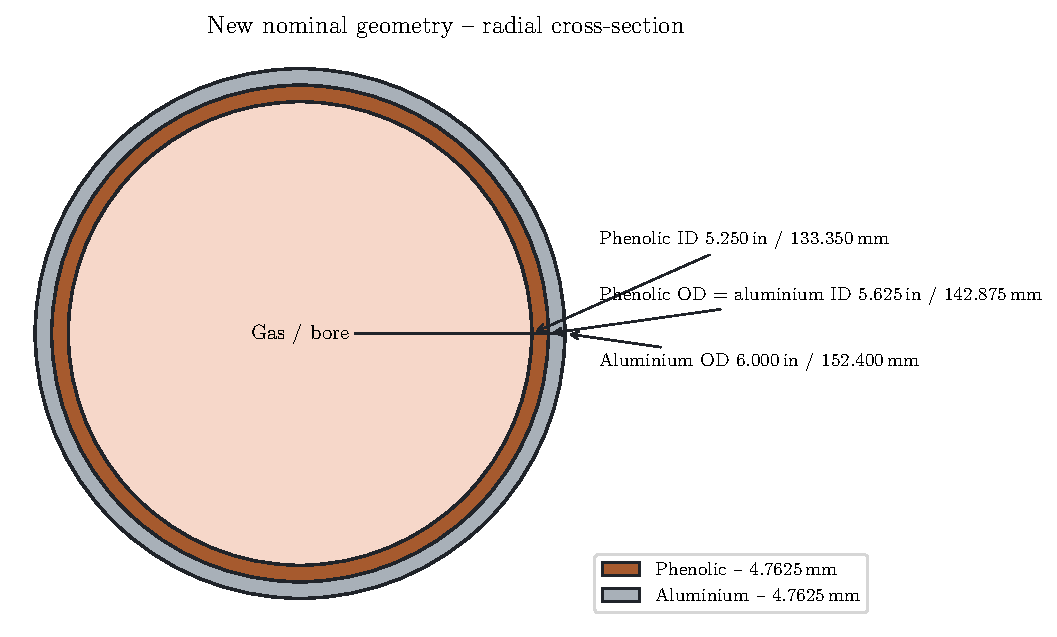
\includegraphics[width=.94\textwidth]{../analysis/newmotor_geometry_en.pdf}
\caption{Nominal two-layer cross-section.}
\end{figure}

As an analytical check, the full \SI{50}{mm} segment contains
\(V_{\mathrm{ph},0}=\SI{1.033208e-4}{m^3}\), or
\(m_{\mathrm{ph},0}=\SI{0.129151}{kg}\) at the reference density
\(\rho_v=\SI{1250}{kg.m^{-3}}\). The corresponding sector mass is
\SI{35.8753}{mg}. These are balance references, not measurements of the
manufactured part.

\subsection{Geometry files}
The \code{geometry/newmotor_phenolic_v0.db} database is a native MAPDL 2026 R1
file containing both glued volumes. It was created on Windows without a mesh
or a \code{SOLVE} command. Its standalone, readable generator,
\code{model/generate_geometry_mapdl.inp}, remains the geometry source. The
exchange database uses global Z as its axis; the analytical solver mesh uses
global Y. A rigid rotation relates them and changes no dimension or thermal
condition.

\section{Computational domain and mesh}
\subsection{Discretization choices}
The mesh is structured, conformal at the interface, and contains only linear
SOLID70 thermal hexahedra. The two materials share interface nodes, so no
contact elements are required. The phenolic has 240 radial rows:
\[
\Delta r_{\mathrm{ph}}=\frac{\SI{4.7625}{mm}}{240}
=\SI{19.84375}{\micro m}.
\]
The aluminium has 64 rows of \SI{74.4141}{\micro m}. The axis is divided into
250 intervals of \SI{0.20}{mm} and the angle into two intervals. Each
potentially exposed phenolic row therefore has 500 faces.

\begin{figure}[H]\centering
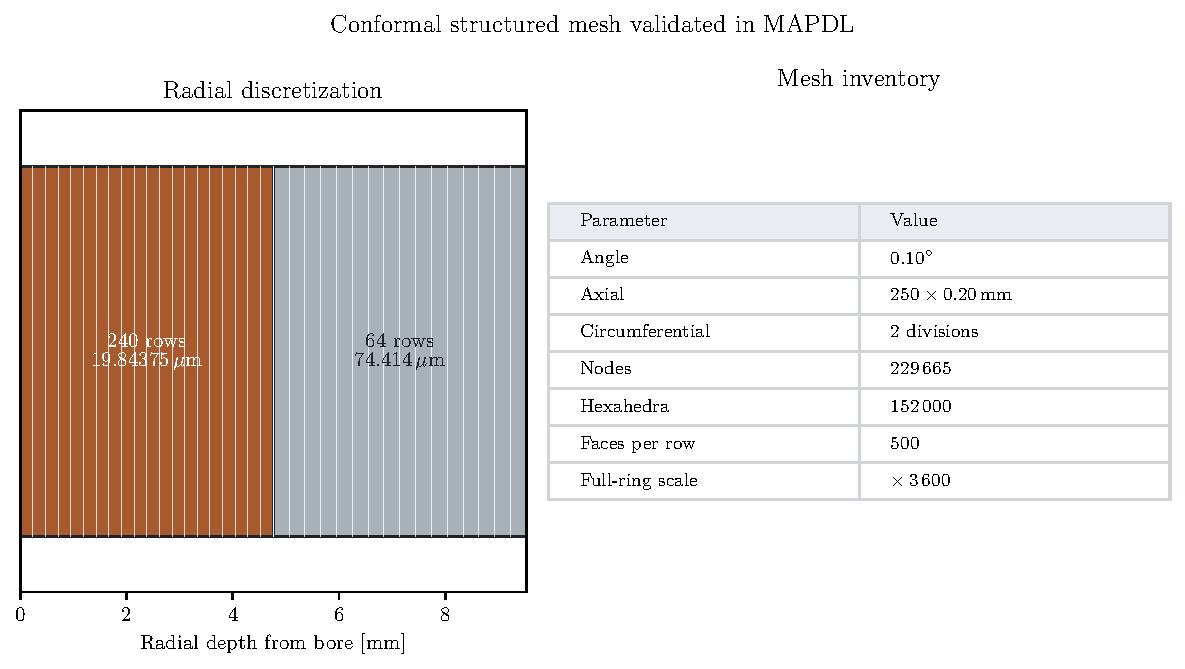
\includegraphics[width=.98\textwidth]{../analysis/newmotor_mesh_en.pdf}
\caption{Radial resolution and final mesh inventory.}
\end{figure}

The final model has 229,665 nodes and 152,000 hexahedra: 120,000 in phenolic
and 32,000 in aluminium. The first 100-division axial mesh produced an aspect
ratio of 25.2 and was archived in the temporary directory. Increasing to 250
divisions reduces the ratio to approximately 10. The final native MAPDL
preflight completes with zero warnings and zero errors.

\subsection{Why a 0.10-degree sector}
Two angular divisions retain three-dimensional topology and explicit
convection faces, while 240 radial rows provide the resolution needed for
progressive removal. The sector cannot represent large-scale circumferential
nonuniformity. It is appropriate for a local axisymmetric response; any crack,
joint, or localized jet requires a wider angular domain.

\section{Planned thermochemical model}
\subsection{Phenolic pyrolysis}
The UserMatTh law retains conversion state variables and returns, for every
live element, conversion \(\alpha\), gas production, and energy terms. Virgin
and char reference densities are \SI{1250}{kg.m^{-3}} and
\SI{600}{kg.m^{-3}}; the provisional pyrolysis enthalpy is
\SI{418}{kJ.kg^{-1}}. Thermal properties depend on temperature and conversion.

The hot face defaults to \(T_g=\SI{2230.85}{\degreeCelsius}\) and
\(h_0=\SI{1000}{W.m^{-2}.K^{-1}}\). Blowing continuously reduces the film
coefficient as gas flux increases. The outer face exchanges with a
\SI{22}{\degreeCelsius} ambient by convection
(\(h=\SI{8}{W.m^{-2}.K^{-1}}\)) and radiation
(\(\varepsilon=0.25\)).

\begin{center}\fbox{\begin{minipage}{0.92\textwidth}\small
\textbf{Qualification limit.} Chamber pressure, gas composition, and carbon
oxidation kinetics are not yet available. The char-consumption law is therefore
explicitly marked \code{EXPLORATORY_NOT_CALIBRATED}. Results may compare
variants and verify balances, but become predictive only after calibration to
the actual material and motor.
\end{minipage}}\end{center}

\subsection{Row removal}
A row is deactivated only after its residual solid mass, following pyrolysis
and carbon consumption, falls below 0.1\,\% of its initial virgin mass. Removal
occurs after acceptance of a converged step and is reapplied after checkpoint
restoration. This replaces the fragile decision based only on average
conversion.

The nominal coupling step is \SI{0.05}{s}; the solver may reduce it to
\SI{0.0005}{s}. The \SI{7}{s} reference horizon is inherited solely for
comparison with the earlier study. A new version must replace it before launch
if the new motor has a different actual burn duration.

\section{Primary quantities and balances}
\subsection{Remaining thickness}
After \(N_k(t)\) rows have been accepted for removal,
\[
s_{\mathrm{removed}}(t)=N_k(t)\,\Delta r_{\mathrm{ph}},\qquad
s_{\mathrm{remaining}}(t)=s_0-s_{\mathrm{removed}}(t),
\quad s_0=\SI{4.7625}{mm}.
\]
The discrete thickness resolution is therefore \SI{19.84375}{\micro m}. The
hot-wall coordinate is \(R_h(t)=R_i+s_{\mathrm{removed}}(t)\).

\subsection{Consumed phenolic mass}
Three quantities must not be conflated:
\begin{enumerate}[nosep]
\item cumulative gas mass produced by pyrolysis;
\item carbon mass consumed at the exposed surface;
\item virgin-equivalent mass of geometrically removed rows.
\end{enumerate}
For a full ring of length \(L\), the last quantity is
\[
m_{\mathrm{removed},0}(t)=\rho_v\,\pi L
\left[\bigl(R_i+s_{\mathrm{removed}}(t)\bigr)^2-R_i^2\right].
\]
The history retains both sector values and values multiplied by 3,600. Every
step closes mass between initial mass, remaining solid, pyrolysis gas, consumed
carbon, and ejected residual. An error beyond tolerance automatically prevents
the next solve.

\subsection{Planned outputs}
The \code{newmotor_v0_history.csv} file is atomically rebuilt after every
accepted step. It includes time, row index, removed and remaining thickness,
sector and full-ring masses, surface temperature, \(\alpha_{\mathrm{mean}}\),
\(\alpha_{\min}\), film coefficient, powers, balance residuals, and warnings.
One immutable JSON record is retained for each checkpoint; the CSV is only a
derived view of those records.

Result plots will be generated from these converged states: remaining and
removed thickness versus time, consumed-mass components, recession rate,
temperature and blowing, radial temperature/conversion profiles, and distance
from the surface to the 90, 95, and 99\,\% pyrolysis fronts. A vertical line
will mark the first numerically meaningful recession front.

\section{Windows execution, pause, and resume}
All large files are isolated in Git-ignored \code{v0/ansystmp}. The \code{v0}
directory is mapped to drive \code{V:} in Windows, and the runtime is
\code{V:\textbackslash ansystmp\textbackslash windows}. It has no reference to
the older project. The UserMatTh source and DLL are copied locally.

Before the first calculation, \code{launch_v0.ps1 -Preflight} verifies input
hashes, mesh, the local \code{1055@localhost} license, and reads the complete
deck without \code{SOLVE}. The September 20, 2026 preflight confirms 229,665
nodes, 152,000 elements, zero warnings, and zero errors. No solver process is
currently active, and no simulation \code{state.json} has been created.

Launch requires explicit \code{-Run} and uses 10 DMP ranks. The script refuses
to start when ANSYS/MPI already exists. Six restart generations are retained.
\code{request_pause.ps1} requests a stop at the next accepted macro-step;
\code{-Run -Resume} is allowed only from a \code{PAUSED_AT_CHECKPOINT} state
whose inputs remain unchanged.

\section{Preparation status and next decisions}
\begin{table}[H]\centering
\begin{tabular}{L{7.2cm}L{5.4cm}}\toprule
Item & Status\\\midrule
Two-volume geometry & created and archived in a native MAPDL database\\
Structured mesh & validated: 229,665 nodes, 152,000 hexahedra\\
Windows preflight & complete, 0 warnings, 0 errors, no solve\\
Solver inputs & sealed with SHA-256\\
Pause/resume & prepared at accepted checkpoints\\
French/English reports & compiled from the same parameters\\
Transient calculation & not started; explicit authorization still required\\\bottomrule
\end{tabular}
\end{table}

Before launch, the actual burn duration, chamber pressure, gas composition,
and measured phenolic properties remain desirable. Without them, v0 is
deliberately a seven-second exploratory reference. Its structure is nonetheless
ready to answer the primary question: how much phenolic was transformed or
removed, and how much sound thickness remains at each time?

\end{document}

